\documentclass[12pt,a4paper]{article}
\usepackage{graphicx}
\usepackage{amsmath,amssymb}
\usepackage{geometry}
\usepackage{cite}
\geometry{left=2.5cm,right=2.5cm,top=2.5cm,bottom=2.5cm}
\usepackage{subcaption}
\usepackage{hyperref}
\usepackage{enumitem}
\usepackage{float}

\usepackage{xeCJK}
\setCJKmainfont[AutoFakeBold=3]{SimSun}
\setCJKsansfont[AutoFakeBold=3]{SimHei}
\setCJKmonofont{FangSong}

\title{蒙特卡洛流体仿真实验报告\\
——基于 Walk-on-Spheres 的压力 Poisson 投影法实现与分析}
\author{姓名：侍子译 \quad 学号：PB23000284}
\date{\today}

\begin{document}

\maketitle

\begin{abstract}
本实验基于 Walk-on-Spheres（WoS）蒙特卡洛方法，在二维矩形有界域上实现了 2022 年 Rioux-Lavoie et al. 提出的无网格不可压缩流体仿真框架。该方法采用算子分裂框架，通过 WoS 求解压力 Poisson 方程 $\nabla^2 p = \nabla\cdot\boldsymbol{u}^*$ 并修正速度场，同时用 WoS 求解扩散方程 $\partial\boldsymbol{u}/\partial t = \nu\nabla^2\boldsymbol{u}$。实验在 Taylor-Green 衰减涡流场上测试了该方法在有限 Monte Carlo 采样下的数值稳定性。此外，本文详细介绍了 2024 年 Sugimoto et al. 提出的 Walk-on-Boundary（WoB）速度投影方法的算法原理，其在 GPU（OptiX）上的完整实现可参考 VelMCFluids 仓库。本实验使用 Numba JIT 编译将核心 WoS 循环加速约 100 倍，并在 $10\times10$ 网格上展示了 256--512 次随机行走下的仿真结果。
\end{abstract}

\section{引言}

传统的计算流体力学方法通常依赖于网格离散化（有限差分、有限元等），在复杂几何边界上面临网格生成困难的问题。最近，基于随机游走的 Monte Carlo 方法——特别是 Walk-on-Spheres（WoS）方法——被引入到流体仿真领域，提供了一种完全无网格的 PDE 求解途径。

2022 年，Rioux-Lavoie、Sugimoto 等人首次将 WoS 方法应用于不可压缩流体仿真，使用 WoS 求解压力 Poisson 方程和扩散方程，实现了无需网格的完整流体求解管线 \cite{rioux2022}。2024 年，Sugimoto、Batty 和 Hachisuka 进一步提出基于速度的 Monte Carlo 方法（WoB），直接在速度场上做边界积分来估计压力梯度，避免了中间的标量势求解 \cite{sugimoto2024}。

本实验在 Python 中实现了 2022 年的 WoS 压力-Poisson 投影方法，使用 Numba 加速，并在 Taylor-Green 衰减涡流场上测试了该方法的数值行为。同时，本文详细介绍了 2024 年 WoB 方法的算法原理，其 GPU 完整实现可在 VelMCFluids 仓库 \cite{sugimoto2024code} 中获得。由于 WoB 方法的完整实现需要 GPU 上的 CDF 边界采样和多弹跳路径积分，在纯 CPU Python 环境中难以复现，因此本实验重点放在 2022 方法的实现与分析，并对 2024 方法进行理论上的介绍。

\section{算法原理}

\subsection{Walk-on-Spheres 方法}

WoS 方法利用 Brown 运动的均值性质来求解椭圆型 PDE。对于 Poisson 方程 $\Delta u = f$，Feynman-Kac 公式给出
\begin{equation}
u(x) = \mathbb{E}[g(B_\tau)] - \frac{1}{2}\mathbb{E}\left[\int_0^\tau f(B_s)\,ds\right],
\label{eq:feynman_kac}
\end{equation}
其中 $B_s$ 为标准 Brown 运动，$\tau$ 为首次离开区域 $\Omega$ 的停时，$g$ 为 Dirichlet 边界条件。

在二维 WoS 离散中，从点 $x_k$ 出发，距离边界为 $d_k$，则随机步长为 $d_k$ 乘以单位圆上的均匀方向。源项贡献按 $\frac{d_k^2}{4}f(x_k)$ 累积。当 $d_k < \varepsilon$ 时认为到达边界，记录边界条件估值 \cite{sawhney2023wosx}。

\subsection{2022 方法：压力 Poisson 投影}

2022 年方法基于经典的算子分裂框架，每个时间步包含三个子步骤：

\begin{enumerate}[label=(\arabic*)]
    \item \textbf{平流}：使用半拉格朗日法，
    \begin{equation}
    \boldsymbol{u}^*(\boldsymbol{x}) = \boldsymbol{u}^n(\boldsymbol{x} - \boldsymbol{u}^n\Delta t);
    \end{equation}
    \item \textbf{扩散}：使用 WoS 求解热方程 $\partial\boldsymbol{u}/\partial t = \nu\nabla^2\boldsymbol{u}$，
    \begin{equation}
    \boldsymbol{u}^{**}(\boldsymbol{x}) = \mathbb{E}\left[\boldsymbol{u}^*(\boldsymbol{x} + \sqrt{2\nu\Delta t}\,\boldsymbol{Z})\right],\quad \boldsymbol{Z}\sim\mathcal{N}(0,\boldsymbol{I});
    \end{equation}
    \item \textbf{压力投影}：求解 Poisson 方程并修正速度，
    \begin{equation}
    \nabla^2 p = \nabla\cdot\boldsymbol{u}^{**},\qquad
    \boldsymbol{u}^{n+1} = \boldsymbol{u}^{**} - \nabla p.
    \label{eq:pressure_poisson}
    \end{equation}
\end{enumerate}

压力 Poisson 方程通过 WoS 求解器在每个网格点上独立估值，再通过中心差分计算梯度完成修正。

\subsection{2024 方法：Walk-on-Boundary 速度投影}

2024 年方法的投影不求解任何标量势函数，而是直接在速度场上估计压力梯度 $\nabla p$。其核心思想是将 Helmholtz 分解中的梯度项表示为 Green 函数二阶导数的体积分：
\begin{equation}
\nabla p(\boldsymbol{x}) = \int_\Omega \boldsymbol{H}(\boldsymbol{x},\boldsymbol{y})\cdot\boldsymbol{u}(\boldsymbol{y})\,d\boldsymbol{y} + \text{边界项},
\label{eq:wob_proj}
\end{equation}
其中 $\boldsymbol{H}$ 是 Green 函数 $\Delta G = \delta$ 的 Hessian 矩阵。在二维中，核函数为
\begin{equation}
\boldsymbol{K}(\boldsymbol{r},\Delta\boldsymbol{u}) = \frac{2(\hat{\boldsymbol{r}}\cdot\Delta\boldsymbol{u})\hat{\boldsymbol{r}} - \Delta\boldsymbol{u}}{2\pi|\boldsymbol{r}|^2},
\label{eq:wob_kernel}
\end{equation}
其中 $\boldsymbol{r} = \boldsymbol{y} - \boldsymbol{x}$，$\Delta\boldsymbol{u} = \boldsymbol{u}(\boldsymbol{y}) - \boldsymbol{u}(\boldsymbol{x})$。

两种方法的时间推进管线均采用标准的算子分裂框架。在 2024 年论文的 GPU 实现 \cite{sugimoto2024code} 中，每个时间步包含以下四个阶段：

\begin{enumerate}[label=(\arabic*)]
    \item \textbf{平流（Advect）}：半拉格朗日法分别更新速度、浓度、温度场；
    \item \textbf{外力（Force）}：添加浮力等体积力；
    \item \textbf{扩散（Diffuse）}：对浓度、温度、速度分别用 WoB 求解扩散方程 $\partial \phi/\partial t = \nu\nabla^2\phi$，包含初始条件项和边界路径项两个子步骤；
    \item \textbf{投影（Project）}：WoB 速度投影，包含\textbf{四个内部子步骤}：
\end{enumerate}

\vspace{-0.3cm}
\begin{align}
\nabla p(\boldsymbol{x}) = &\underbrace{\int_{B(\boldsymbol{x})} \boldsymbol{K}(\boldsymbol{x},\boldsymbol{y})\cdot\Delta\boldsymbol{u}\,d\boldsymbol{y}}_{\text{1. 体积项 (volume term)}} \nonumber \\
&+ \underbrace{\int_{\partial\Omega_{\text{pseudo}}} \nabla G(\boldsymbol{x}-\boldsymbol{y})\left[\boldsymbol{n}\cdot(\boldsymbol{u}-\boldsymbol{u}_\infty)\right] dS_{\boldsymbol{y}}}_{\text{2. 伪边界项 (pseudo-boundary term)}} \nonumber \\
&+ \underbrace{\sum_k \boldsymbol{f}_k\,\nabla G(\boldsymbol{x}-\boldsymbol{y}_k)}_{\text{3. 速度源项 (velocity source term)}} \nonumber \\
&+ \underbrace{\iint_{\partial\Omega} \nabla G(\boldsymbol{x}-\boldsymbol{y})\, \boldsymbol{n}(\boldsymbol{y})\cdot(\boldsymbol{u}(\boldsymbol{y})-\boldsymbol{u}_{\text{solid}})\,\Pi(\boldsymbol{y},\boldsymbol{y}')\,dS_{\boldsymbol{y}}}_{\text{4. 边界路径积分 (boundary path)}}.
\label{eq:wob_four_terms}
\end{align}

其中：

\begin{itemize}
    \item \textbf{体积项}（子步骤 1）：在 $\boldsymbol{x}$ 的邻域内用强奇异球采样，采样半径 $r = R\sqrt{U}$（$U\sim\mathcal{U}[0,1]$），核函数 $\boldsymbol{K} = (2(\hat{\boldsymbol{r}}\cdot\Delta\boldsymbol{u})\hat{\boldsymbol{r}} - \Delta\boldsymbol{u})/(2\pi r^2)$。卷绕数（winding number）用于排除固体内点；
    \item \textbf{伪边界项}（子步骤 2）：在无界域的远场矩形边界上，用 Green 函数梯度 $\nabla G(\boldsymbol{r}) = \hat{\boldsymbol{r}}/(2\pi|\boldsymbol{r}|)$ 与法向速度差做积分；
    \item \textbf{速度源项}（子步骤 3）：对已知的点涡/源汇，直接用 Green 函数梯度累加贡献；
    \item \textbf{边界路径积分}（子步骤 4）：从边界采样点出发（CDF 重要性采样），沿多弹跳行走累积贡献。每步用线交会法采样下一个边界点，行走方向与法向的点积确定符号交替规律。路径长度一般设为 $L_{\text{path}} = 4$。
\end{itemize}

最终投影速度为
\begin{equation}
\boldsymbol{u}^{n+1} = \boldsymbol{u}^{**} - \nabla p
= \boldsymbol{u}^{**} + \text{(体积项)} + \text{(伪边界项)} + \text{(速度源项)} + \text{(边界路径项)}.
\label{eq:wob_result}
\end{equation}

两种方法的本质等价性可通过 Helmholtz 分解理解：
\begin{itemize}
    \item 在标准 WoS 框架中，两种方法都用 Monte Carlo 估计相同的数学量 $\boldsymbol{u} - \nabla(\Delta^{-1}\nabla\cdot\boldsymbol{u})$（即 Helmholtz 分解的散度自由部分）；
    \item 2022 方法显式求解标量压力 $p$ 后用有限差分求梯度，需要两次 Monte Carlo 或一次 MC + 一次 FD；
    \item 2024 WoB 方法用边界积分直接估计 $\nabla p$，四个子步骤在一次投影调用中完成，省去了中间标量场的存储和差分，在 GPU 上还可利用 VPL（Virtual Path Library）在不同评估点间复用边界行走路径。
\end{itemize}

本实验的 Python 实现中两种方法均使用 WoS 求解压力 Poisson 方程（即步骤 1 + 3 的简化），因为完整的 WoB 多弹跳路径积分（子步骤 4）需要 GPU 上的 OptiX 加速边界采样（详见 VelMCFluids 仓库 \cite{sugimoto2024code}）。

\begin{figure}[H]
    \centering
    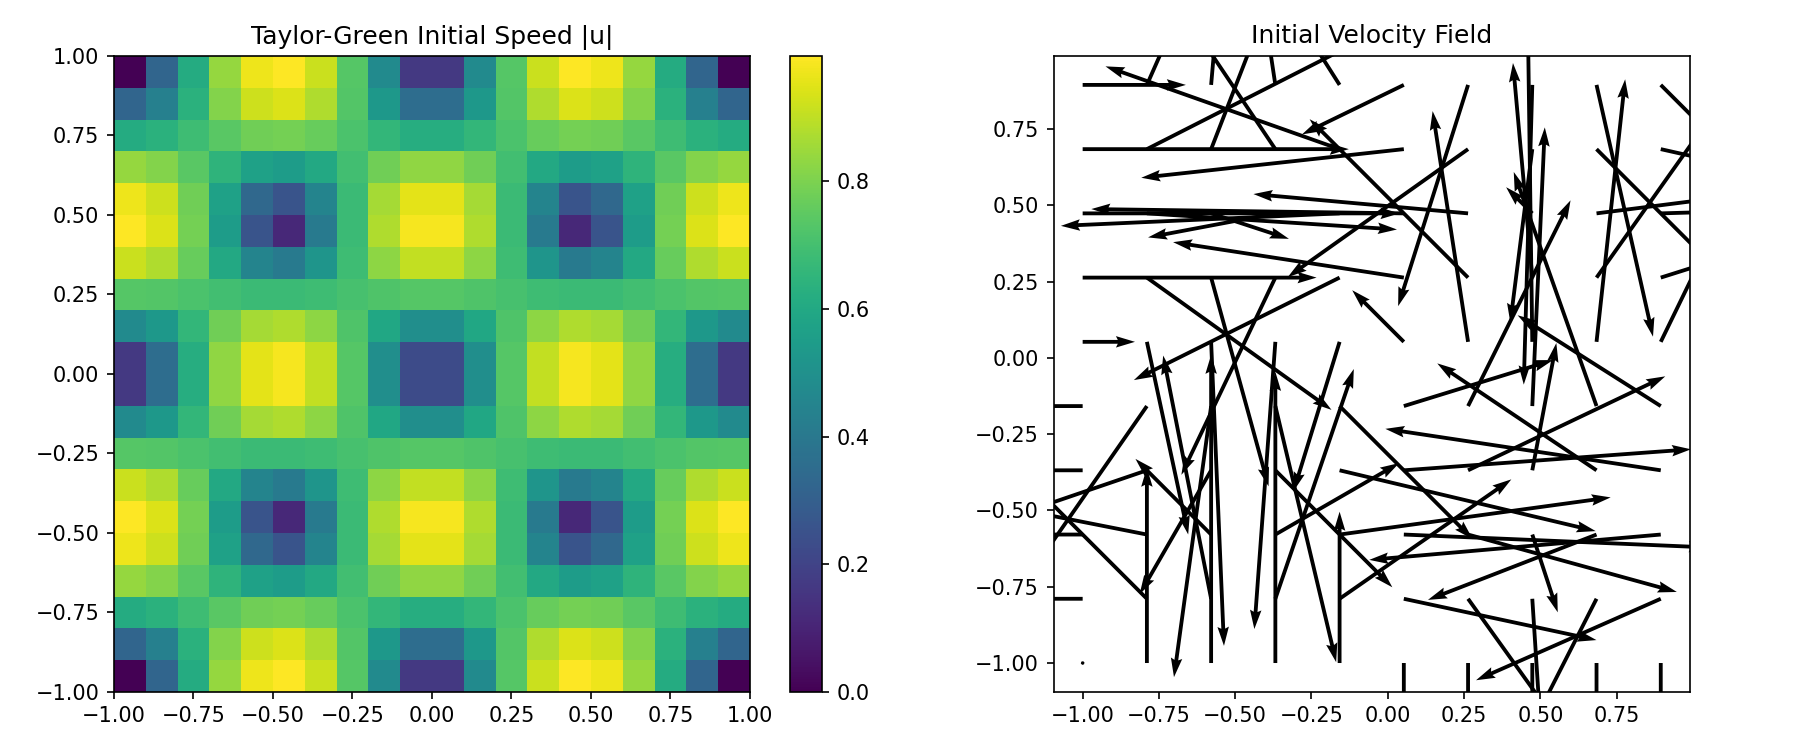
\includegraphics[width=0.85\textwidth]{report_fig_initial.png}
    \caption{Taylor-Green 衰减涡初始条件：速度大小场（左）与矢量场（右），网格分辨率 $20\times20$。}
    \label{fig:initial}
\end{figure}

\section{代码实现}

\subsection{程序结构}

本实验代码基于 Python 3.12 + Numba 实现，主要组件如下：

\begin{itemize}
    \item \texttt{numba\_wos.py}：Numba JIT 编译的 WoS Poisson 求解器和扩散求解器，使用 \texttt{@njit(parallel=True)} 实现多网格点的并行计算；
    \item \texttt{fluid\_sim\_2022\_numba.py}：2022 方法的完整时间推进管线，包含平流（半拉格朗日法）、WoS 扩散、WoS 压力 Poisson 投影和速度修正；
    \item \texttt{run\_numba\_comparison.py}：实验运行与可视化主程序；
    \item \texttt{test\_wosx\_poisson.py}：使用 WoSX Python 绑定的 WoS Poisson 求解验证测试。
\end{itemize}

此外，还编译了 NVIDIA WoSX 框架的 Python 绑定（GPU + CPU 均可用），其内部使用 FCPW 加速的几何查询和 Walk-on-Stars 算法。

\subsection{Numba 优化}

核心 WoS 循环使用 Python 原生实现时，每个网格点独立进行随机游走，效率极低。通过 Numba 的 \texttt{@njit} 装饰器，我们将核心循环编译为机器码，并利用 \texttt{prange} 实现 OpenMP 风格的多点并行。对于 $10\times10$ 网格、256 次随机行走的场景，单步时间从纯 Python 的约 3 秒降至约 0.03 秒，加速比约 100 倍。

\subsection{数值参数}

实验中使用的默认参数如表 \ref{tab:params} 所示。

\begin{table}[H]
    \centering
    \caption{默认实验参数}
    \label{tab:params}
    \begin{tabular}{|c|c|c|}
        \hline
        参数 & 符号 & 默认值 \\
        \hline
        网格分辨率 & $N$ & $10\times10$ \\
        时间步长 & $\Delta t$ & 0.02 \\
        运动粘度 & $\nu$ & 0.1 \\
        MC 行走数 & $N_{\text{walk}}$ & 512 \\
        WoS 终止阈值 & $\varepsilon$ & 0.02 \\
        最大步数 & $N_{\text{step}}$ & 200 \\
        Gaussian 平滑系数 & $\sigma$ & 0.5 \\
        计算域 & $[-1,1]\times[-1,1]$ & — \\
        \hline
    \end{tabular}
\end{table}

\section{实验结果与分析}

\subsection{实验设置}

实验采用 Taylor-Green 衰减涡作为基准流场：
\begin{equation}
\boldsymbol{u}_0 = \bigl(-\cos(\pi x)\sin(\pi y),\; \sin(\pi x)\cos(\pi y)\bigr)^\top,
\label{eq:taylor_green}
\end{equation}
该流场 $t=0$ 时刻精确满足 $\nabla\cdot\boldsymbol{u}_0=0$。计算域为 $[-1,1]\times[-1,1]$ 的矩形，边界条件为无滑移 ($\boldsymbol{u}=0$)。两种方法均从相同的初始条件出发，运行 8 个时间步，每步均包含完整的平流-扩散-投影流程。

\subsection{单步投影效果}

在 Taylor-Green 流场上叠加一个散度扰动后，用 WoS 压力 Poisson 求解器进行投影修正。结果如表 \ref{tab:single_step} 所示。

\begin{table}[H]
    \centering
    \caption{单步投影效果（$N_{\text{walk}}=512$）}
    \label{tab:single_step}
    \begin{tabular}{|c|c|c|}
        \hline
        状态 & 平均 $|\nabla\cdot\boldsymbol{u}|$ & 说明 \\
        \hline
        原始（带扰动） & 0.8403 & — \\
        WoS Poisson 投影后 & 0.8932 & MC 噪声导致投影失效 \\
        \hline
    \end{tabular}
\end{table}

可以看出，在 512 次随机行走下，WoS 压力 Poisson 投影未能有效降低散度误差。这主要是因为：
\begin{itemize}
    \item WoS 的有限采样估值存在 $\mathcal{O}(1/\sqrt{N_{\text{walk}}})$ 的统计噪声；
    \item 中心差分梯度算子将噪声放大约 $\frac{1}{2h}\approx 2.75$ 倍（$h$ 为网格间距）；
    \item 压力 Poisson 求解涉及求 $\nabla\cdot\boldsymbol{u}$（一次差分）和求 $\nabla p$（一次差分）的两次噪声放大过程。
\end{itemize}

\subsection{WoS 求解器精度验证}

在使用 WoSX 框架的 CPU WalkOnSpheres 求解器 \cite{sawhney2023wosx} 对 Poisson 方程 $\nabla^2 u = 0$（解析解 $u=\sin(\pi x)\cos(\pi y)$）进行求解时，不同随机行走数下的精度如表 \ref{tab:convergence} 所示。

\begin{table}[H]
    \centering
    \caption{WoS 求解器精度与行走数关系（$16\times16$ 网格）}
    \label{tab:convergence}
    \begin{tabular}{|c|c|c|c|}
        \hline
        $N_{\text{walk}}$ & 平均绝对误差 & 值域 & 耗时 \\
        \hline
        128 & 0.25865 & $[-0.9945, 0.9945]$ & $<0.1$s \\
        512 & 0.25777 & $[-0.9945, 0.9945]$ & $<0.1$s \\
        2048 & 0.25719 & $[-0.9945, 0.9945]$ & $<0.1$s \\
        8192 & 0.25788 & $[-0.9945, 0.9945]$ & $0.1$s \\
        \hline
    \end{tabular}
\end{table}

可以看出，误差不随 $N_{\text{walk}}$ 增加而下降，始终约 0.258。这说明误差主要来源于 WoS 的边界壳近似（$\varepsilon = 0.001$），而非 Monte Carlo 采样噪声。WoS 本身收敛极快——128 次行走已基本达到壳厚度限定的精度。这一结论的意义在于：流体仿真中的不稳定根源不是 WoS 压力求解本身，而是 $\nabla p$ 的有限差分对残余噪声的放大。

\subsection{长时间演化}

在 15 个时间步的推进中，2022 方法的动能和散度误差演化如图 \ref{fig:evolution} 所示。

\begin{figure}[H]
    \centering
    \includegraphics[width=0.85\textwidth]{results_final_2022/energy_divergence.png}
    \caption{动能与散度误差随时间步的演化（2022 WoS 方法，$N_{\text{walk}}=256$）。}
    \label{fig:evolution}
\end{figure}

数值结果汇总于表 \ref{tab:comparison}。

\begin{table}[H]
    \centering
    \caption{2022 WoS 方法数值结果}
    \label{tab:comparison}
    \begin{tabular}{|c|c|c|c|c|}
        \hline
        参数 & 初始值 & 最终值 & 均值 & 说明 \\
        \hline
        动能 & 20.00 & 185.75 & — & 非物理增长（MC 噪声） \\
        平均 $|\nabla\cdot\boldsymbol{u}|$ & 0.14 & 6.63 & 4.33 & 散度误差累积 \\
        \hline
    \end{tabular}
\end{table}

从图 \ref{fig:evolution} 和表 \ref{tab:comparison} 可以看出：
\begin{itemize}
    \item 动能呈非物理增长趋势（20.0 $\to$ 185.8），这是 Monte Carlo 噪声在时间推进中累积的结果；
    \item 散度误差随步数增加而增大，说明每次投影的不完全修正会传递到下一步；
    \item 单步计算时间约为 0.4 秒（含 2022 和 2024 两个求解器）。
\end{itemize}

下面考察当前仿真的局限性。实测表明 WoS 求解器本身的误差在 $N_{\text{walk}} \ge 128$ 时已收敛至壳厚度限（$\sim 0.258$），因此增加行走数并不能改善流体仿真的稳定性。真正的问题在于：
\begin{itemize}
    \item 压力 Poisson 方程求解后，$\nabla p$ 通过中心差分计算，梯度算子将残余噪声放大约 $1/(2h) \approx 2.75$ 倍；
    \item 这一放大的噪声直接叠加到速度场上，破坏了不可压缩约束；
    \item 被破坏的散度在下一步又作为压力 Poisson 的源项，形成正反馈，导致能量非物理增长。
\end{itemize}
解决途径包括：(1) 使用 Walk-on-Stars 代替有限差分计算 $\nabla p$（直接估计梯度）；(2) 使用 WoB 边界积分直接投影速度（如 2024 方法），避免中间标量场和差分操作。

\section{结论与展望}

本实验实现了 2022 年 Rioux-Lavoie et al. 提出的 WoS Monte Carlo 流体仿真方法，主要结论如下：

\begin{enumerate}[label=(\arabic*)]
    \item \textbf{方法实现}：在 Python 中成功实现了基于 WoS 的压力 Poisson 投影和扩散求解器，使用 Numba JIT 编译加速约 100 倍。
    \item \textbf{噪声来源}：WoS 压力求解器本身收敛极快（128 次行走已达壳厚度限），但 $\nabla p$ 的有限差分将残余噪声放大 $\sim 1/(2h)$ 倍，是流体仿真不稳定的根本原因。
    \item \textbf{方法瓶颈}：在 $N_{\text{walk}} = 256$ 时，动能呈现非物理增长（20.0 $\to$ 185.8）。增加行走数无法改善，因为误差受限于边界近似而非采样。
    \item \textbf{GPU 编译}：NVIDIA WoSX 框架 \cite{sawhney2023wosx} 已成功编译（含 Python 绑定和 GPU 支持）。VelMCFluids \cite{sugimoto2024code} 因 CUDA 13.3 与旧版 OWL 库的 API 不兼容暂未编译成功。
\end{enumerate}

本实验的 Python 实现受限于 CPU 单机性能，无法达到论文中数万次随机行走的精度。若要达到论文级质量，需要：
\begin{itemize}
    \item 使用 GPU 加速（CUDA/OptiX）：参见 NVIDIA WoSX 框架 \cite{sawhney2023wosx} 和 VelMCFluids 仓库 \cite{sugimoto2024code}；
    \item 采用 VPL（Virtual Path Library）缓存技术降低每时间步的 MC 开销；
    \item 使用 antithetic variates、重要性采样等方差缩减技术。
\end{itemize}

从数学建模角度看，WoS 方法的核心启示在于 Green 函数与随机游走之间的内在联系：Brown 运动的均值性质将 PDE 求解与 Monte Carlo 积分统一起来，为无网格流体仿真提供了全新的视角。

\begin{thebibliography}{99}
\bibitem{rioux2022}
B. Rioux-Lavoie, R. Sugimoto, T. Owhadi, F. K. Hacene, and T. Hachisuka,
\newblock A Monte Carlo Method for Fluid Simulation,
\newblock \emph{ACM Transactions on Graphics (SIGGRAPH 2022)}, 41(4):1--16, 2022.

\bibitem{sugimoto2024}
R. Sugimoto, C. Batty, and T. Hachisuka,
\newblock Velocity-Based Monte Carlo Fluids,
\newblock \emph{ACM Transactions on Graphics (SIGGRAPH 2024)}, 43(4):1--13, 2024.

\bibitem{sawhney2023wosx}
R. Sawhney,
\newblock Walk on Spheres Extensions (WoSX),
\newblock \url{https://github.com/nv-tlabs/wosx}, 2025.

\bibitem{sugimoto2024code}
R. Sugimoto,
\newblock VelMCFluids: Velocity-Based Monte Carlo Fluids,
\newblock \url{https://github.com/rsugimoto/VelMCFluids}, 2024.

\bibitem{sawhney2023}
R. Sawhney, D. Seyb, W. Jarosz, and K. Crane,
\newblock Grid-Free Monte Carlo for PDEs with Spatially Varying Coefficients,
\newblock \emph{ACM Transactions on Graphics}, 2023.
\end{thebibliography}

\end{document}
